\chapter{Comparison among all categories of constraints.}
\label{ch:comp}
\begin{table}
\hspace{-2cm}
\begin{tabular}{|l|l|l|l|l|}
	\hline
	Input Program  &  C1 & C2 & C3 & C4 \\
	\hline
\begin{lstlisting}[language=Python]
#'a' is a local var
a = x
while w:
	y = a
	a = z
z = y
\end{lstlisting}&
\begin{lstlisting}
x <= a
a + w <= y
z + w <= a
y <= z
\end{lstlisting}&
\begin{lstlisting}
x <= a
a + x + w <= y
a + x + z + w <= a
a + x + z + w <= y
a + x + z + y + w <= z
y + x + w <= z
\end{lstlisting}&
\begin{lstlisting}
x + w <= y
x + z + w <= y
y <= z	
\end{lstlisting}&
\begin{lstlisting}
x + w <= y
x + z + w <= y
y + x + w <= z
y + x + z + w <= z	
\end{lstlisting}\\
	\hline
	
\end{tabular}
\caption{Example for comparison}
\label{tbl:compex}
\end{table}


Example given in table \ref{tbl:compex} is suitable to differentiate between all category.
First algorithm fails to track information flow w\marr z in last statement z = y.
Second algorithm is able to track information flow w\marr z in last statement z = y but it will show additional false information flow z \marr y too. 
Third algorithm avoids tracking of additional false information flow z \marr y but it fails to show information flow w \marr z because of PC reset.
Fourth analysis avoids tracking of false information flow as well as tracks information flow caused by nonterminating loop( w \marr z). Table \ref{tbl:compcopy} shows constraints generated for copy program given in Denning,s book by all constraint generator.
\begin{table}
\hspace{-2cm}
\begin{tabular}{|l|l|l|l|l|}
	\hline
	Programs  &  C1 & C2 & C3 & C4 \\
	\hline
	Copy1&
	\begin{lstlisting}
	x <= z
	z <= y
	\end{lstlisting}&
	\begin{lstlisting}
	x <= z
	x + z <= y
	\end{lstlisting}&
	\begin{lstlisting}
	x <= y
	\end{lstlisting}&
	\begin{lstlisting}
	x <= y
	\end{lstlisting}\\
	\hline
	Copy2&
	\begin{lstlisting}
	Low <= z
	Low <= y
	y + z <= y
	y + x + z <= z
	y + z <= z
	\end{lstlisting}&
	\begin{lstlisting}
	Low <= z
	Low <= y
	y + z <= y
	y + x + z <= z
	y + z <= z
	y + x + z <= y
	\end{lstlisting}&
	\begin{lstlisting}
	Low <= y
	y <= y
	y + x <= y
	\end{lstlisting}&
	\begin{lstlisting}
	Low <= y
	y <= y
	y + x <= y
	\end{lstlisting}
	\\
	\hline
	Copy3&
	\begin{lstlisting}
	x + s0 <= s0
	x + s1 <= s1
	s0 <= s0
	Low <= y
	s1 <= s1
	\end{lstlisting}&
	\begin{lstlisting}
	x + s0 <= s0
	x + s1 <= s1
	s0 <= s0
	s0 <= y
	s1 + s0 <= s1
	s1 <= s1
	s1 <= y
	s1 + s0 <= s0
	\end{lstlisting}&
	\begin{lstlisting}
	x + s0 <= s0
	x + s1 <= s1
	s0 <= s0
	Low <= y
	s1 <= s1
	\end{lstlisting}&
	\begin{lstlisting}
	x + s0 <= s0
	x + s1 <= s1
	s0 <= s0
	s0 <= y
	s1 + s0 <= s1
	s1 <= s1
	s1 <= y
	s1 + s0 <= s0
	\end{lstlisting}
	\\
	\hline
	Copy4&
	\begin{lstlisting}
	x <= e0
	x <= e1
	Low <= y
	Low <= e1
	Low <= e0
	\end{lstlisting}&
	\begin{lstlisting}
	x <= e0
	x <= e1
	e0 <= y
	e0 <= e1
	e1 <= y
	e1 <= e0
	\end{lstlisting}&
	\begin{lstlisting}
	x <= e0
	x <= e1
	Low <= y
	Low <= e1
	Low <= e0
	\end{lstlisting}&
	\begin{lstlisting}
	x <= e0
	x <= e1
	e0 <= y
	e0 <= e1
	e1 <= y
	e1 <= e0
	\end{lstlisting}
	\\
	\hline
	Copy5&
	\begin{lstlisting}
	Low <= y
	\end{lstlisting} &
	\begin{lstlisting}
	Low <= y
	x <= y
	\end{lstlisting}&
	\begin{lstlisting}
	Low <= y 
	\end{lstlisting}&
	\begin{lstlisting}
	Low <= y
	x <= y
	\end{lstlisting}\\
	\hline
	Copy6&
	\begin{lstlisting}
	Low <= z
	Low <= sum
	Low <= y
	x + sum + z <= sum
	y + z <= y
	\end{lstlisting}&
	\begin{lstlisting}
	Low <= z
	Low <= sum
	Low <= y
	x + sum + z <= sum
	y + x + sum + z <= y
	y + x + sum + z <= sum
	\end{lstlisting} &
	\begin{lstlisting}
	Low <= y
	y <= y  
	\end{lstlisting}&
	\begin{lstlisting}
	Low <= y
	y + x <= y
	\end{lstlisting}\\
	\hline
	Dynamic label&
	\begin{lstlisting}
	x <= a
	a <= y
	z <= a
	\end{lstlisting}&
	\begin{lstlisting}
	x <= a
	a + x <= y
	a + x + z <= a
	\end{lstlisting} &
	\begin{lstlisting}
	x <= y
	\end{lstlisting}&
	\begin{lstlisting}
	x <= y
	\end{lstlisting}\\
	\hline
\end{tabular}
\label{tbl:compcopy}
\caption{Constraints generated by all four algorithm for copy programs given Denning \cite{denning}}
\end{table}
	\begin{figure*}[h]
		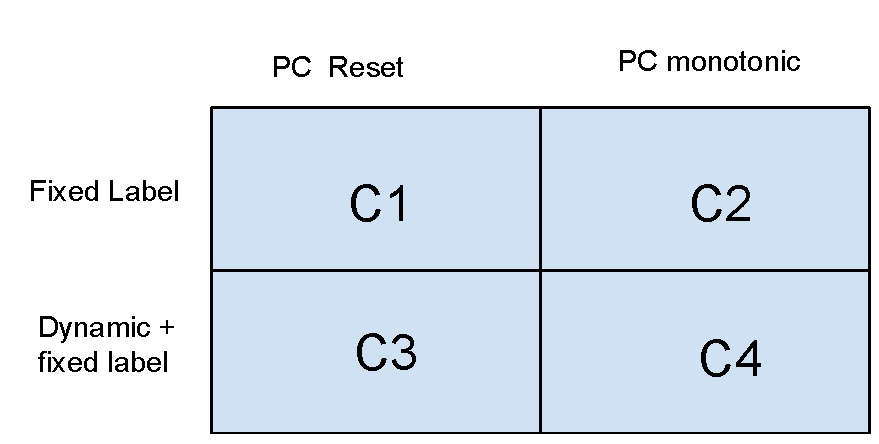
\includegraphics[width=0.6\textwidth]{category}
		\centering
		\caption{Category of constraint generator}
		\label{fig:set}
	\end{figure*}
	\begin{figure*}[h]
		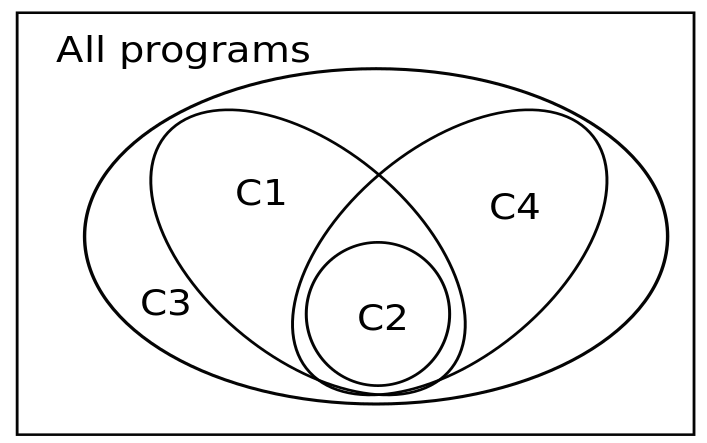
\includegraphics[width=0.6\textwidth]{rsz_set}
		\centering
		\caption{Set diagram}
		\label{fig:set}
	\end{figure*}
	Figure \ref{fig:set} shows the relationship between set of programs declared secure by all constraint generator. C1-C4 are abbreviation for category 1 - category 4. Number of constraints is inversely proportional to size of set of program declared secure, because more constraints means high probability of violation of security. In category 1 generator generates many false constraints because of absence of dynamic label, but category 3 uses dynamic labels with fixed so it reduces number of constraints. Constraints generated by category 1 are superset of constraints generated by category 3 this relationship shows that set of program declared secure by C1 must be subset of C3. Similarly C2 and C4 differ by use of dynamic labels so set of accepted program by C2 is a subset of set of programs accepted by C4. Use of monotonic PC label helps to capture global information flows so use of monotonic PC label increases the number of constraints. C3 and C4 differ by use of PC label scheme, C4 using monotonic PC and C3 using PC reset so constraints generated by C4 are superset of constraints generated by C3 so set of accepted programs of C4 must be subset of C3. Similarly C2 and C1 differ by PC label scheme so set of accepted programs is a subset of set of programs accepted by C1.    
	\begin{figure}
		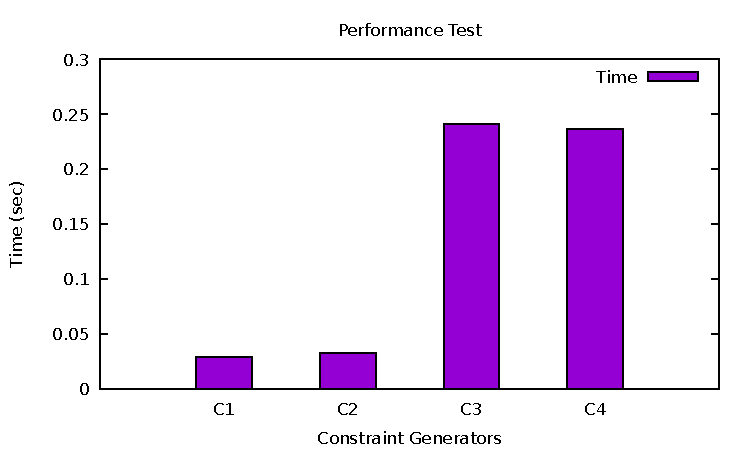
\includegraphics[width=1\textwidth]{graph.pdf}
		\centering
		\caption{Performance test}
		\label{fig:ptest}
	\end{figure}
	\pagebreak
	Figure \ref{fig:ptest} shows the average time taken in processing one copy program by all four generator. 
	Time taken in order C1 < C2 < C4 < C3. C4 taking little less time than C3 because of optimization in label generation, this optimization uses property of monotonic PC so it can not applied in C3.